\documentclass[12pt,a4paper]{report}

% Compile with XeLaTeX (twice, to update the table of contents)
%================================================
% ENCODING & LANGUAGE
%================================================
\usepackage{fontspec}
\usepackage{polyglossia}
\setmainlanguage{english}
\setotherlanguage{vietnamese}

\setmainfont{Times New Roman}[
    UprightFont = *,
    BoldFont = * Bold,
    ItalicFont = * Italic,
    BoldItalicFont = * Bold Italic,
    Ligatures = TeX
]

\usepackage{ragged2e} % Flexible text alignment (justify, ragged)

%================================================
% PAGE LAYOUT
%================================================
\usepackage{geometry}
\geometry{
    a4paper,
    left=2.5cm,
    right=2.5cm,
    top=2cm,
    bottom=2cm
}

\setlength{\headheight}{14.5pt}

\usepackage{setspace}
\setstretch{1.3}            % Line spacing
\parindent=1.25cm           % Paragraph indentation
\setlength{\parskip}{6pt}   % Space between paragraphs

%================================================
% HEADERS & FOOTERS
%================================================
\usepackage{fancyhdr}
\fancyhf{}

\fancyfoot[R]{\thepage}

\renewcommand{\headrulewidth}{0pt}
\renewcommand{\footrulewidth}{0pt}

\pagestyle{fancy}

\fancypagestyle{plain}{
    \fancyhf{}
    \fancyfoot[R]{\thepage}
    \renewcommand{\headrulewidth}{0pt}
    \renewcommand{\footrulewidth}{0pt}
}

%================================================
% TITLES, TABLE OF CONTENTS & LISTS
%================================================
\usepackage{titlesec}
\usepackage{tocloft}

% Chapter style
\titleformat{\chapter}[hang]
  {\bfseries\LARGE}
  {Chapter \thechapter:}{1em}{}
\titlespacing*{\chapter}{0pt}{0pt}{15pt}

% Section style
\titleformat{\section}
  {\bfseries\Large}
  {\thesection}{0.8em}{}
\titlespacing*{\section}{0pt}{10pt plus 2pt minus 1pt}{6pt}

% Subsection style
\titleformat{\subsection}
  {\bfseries\normalsize}
  {\thesubsection}{0.8em}{}
\titlespacing*{\subsection}{0pt}{8pt plus 1pt minus 1pt}{4pt}

% TOC spacing
\setlength{\cftbeforechapskip}{0.5em}

%================================================
% GRAPHICS & HYPERLINKS
%================================================
\usepackage{graphicx}
\usepackage{caption}
\usepackage{float}

\usepackage[hyphens]{url}   % Allow line breaks in long URLs
\usepackage{microtype}      % Improved justification and line breaking
\Urlmuskip=0mu plus 1mu\relax

\usepackage{hyperref}
\hypersetup{
    colorlinks=true,
    linkcolor=black,
    urlcolor=blue,
    citecolor=black,
    pdfborder={0 0 0}
}

\sloppy                    % Relax line breaking to avoid warnings
\captionsetup{font=it}     % Italic captions

%================================================
% ADDITIONAL UTILITIES
%================================================
\usepackage{amsmath, amssymb} % Math symbols
\usepackage{booktabs}         % Professional tables
\usepackage{array}            % Custom column formatting
\usepackage{xcolor}           % Color support
\usepackage{enumitem}         % List customization

\setlist{nosep, leftmargin=1.25cm}


\setlength{\parindent}{0pt}
\newcolumntype{L}[1]{>{\RaggedRight\arraybackslash}p{#1}}

% Figure helper: shows the image if the file exists, otherwise a visible
% placeholder, so the report compiles while evidence is still missing.
% Usage: \evfig{file}{width}{caption}{label}
\newcommand{\evfig}[4]{%
  \begin{figure}[H]
    \centering
    \IfFileExists{images/#1}{%
      \includegraphics[width=#2\textwidth]{images/#1}%
    }{%
      \fbox{\parbox[c][4cm][c]{0.7\textwidth}{\centering
        \textbf{[TODO: evidence missing]}\\ \texttt{\detokenize{#1}}}}%
    }
    \caption{#3}
    \label{#4}
  \end{figure}%
}

% Marks text that must be filled in once Exercise 1 is verified.
\newcommand{\todo}[1]{\textcolor{red}{\textbf{[TODO: #1]}}}

\begin{document}

\pagenumbering{roman}
\begin{titlepage}
\begin{center}

{\bfseries\large VIETNAM NATIONAL UNIVERSITY HO CHI MINH CITY}\\[0.15cm]
{\bfseries\Large UNIVERSITY OF INFORMATION TECHNOLOGY}\\[0.15cm]

\vspace*{\fill}


\includegraphics[scale=0.6]{images/logouit.png}

\vspace*{\fill}

{\bfseries\fontsize{19}{21}\selectfont HOMEWORK - LAB 03}\\[0.3cm]
{\large Drum Machine, Grand Piano 88 and PVS Arena}

\vspace*{\fill}

\begin{tabular}{rl}
\textbf{Lecturer:} & Nguyễn Thanh Bình - Trần Vĩnh Khiêm\\
\textbf{Name:}& Quảng Phú Hưng\\
\textbf{Student ID:}& 24520626 \\
\textbf{Class:} & MSIS207.R12.CTTT\\
\textbf{Course:} & 2026--2027\end{tabular}

\vspace*{\fill}

{\bfseries Ho Chi Minh City, November 12, 2026}

\end{center}
\end{titlepage}

\tableofcontents
\addcontentsline{toc}{chapter}{Table of Contents}
\clearpage

\clearpage
\pagenumbering{arabic}

\chapter{Homework 1: Drum Machine}
\label{chap:hw1}

7 keyboard drum pads (\texttt{e.code}, no key repeat), polyphonic playback, hit log, level meter, plus Controls (kit, volume, mute) and a Looper (record, overdub, loop/once, speed).

\section{Evidence}

\evfig{hw1_lighthouse.png}{0.9}{Lighthouse on the production build: Performance 100, Accessibility 100, Best Practices 100, SEO 91}{fig:hw1-lh}
\evfig{hw1_a11y.png}{0.9}{Accessibility tree of the Looper region: named buttons, \texttt{progressbar}, \texttt{status}}{fig:hw1-a11y}

\section{Verification}

\begin{table}[H]
\centering
\begin{tabular}{L{5.5cm} L{7.5cm}}
\toprule
\textbf{Check} & \textbf{Result} \\
\midrule
\texttt{npm test} & 15 files, 146 tests pass \\
\texttt{npm run lint} & Clean \\
Contrast (WCAG 1.4.3, 1.4.11) & 16/16 pairs pass, lowest 6.24:1 \\
Lighthouse Performance & 69 (dev server) $\rightarrow$ 100 (build) \\
Lighthouse Accessibility & 100 \\
\bottomrule
\end{tabular}
\caption{Homework 1 results}
\label{tab:hw1-verify}
\end{table}

Not done: Lighthouse JSON export, 375 px and keyboard-tab screenshots, screen reader test. The Performance drop to 69 was caused by AI-added Google Fonts and eager WAV preloading (AI failure audit, error 5); fixed and re-measured.

\section{Source Code}

\begin{center}
    \href{https://github.com/Prosperum26/24520626_QuangPhuHung_MSIS207_Lab03/tree/main/src/homeworks/DrumMachine}
    {\textbf{View Homework 1 on GitHub}}
\end{center}

\chapter{Homework 2: Grand Piano 88}
\label{chap:hw2}

88-key piano (52 white, 36 black), polyphonic synth with at most 8 voices and FIFO voice stealing, memoized keys, and a recorder with abortable replay at 0.5x, 1x and 2x.

\section{Evidence}

\evfig{hw2_lighthouse.png}{0.9}{Lighthouse on the production build: Performance 100, Accessibility 100, Best Practices 100, SEO 91}{fig:hw2-lh}
\evfig{hw2_profiler.png}{0.9}{React Profiler: one key press re-renders one \texttt{PianoKey} (reason: \texttt{isPressed})}{fig:hw2-profiler}
\evfig{hw2_steal.png}{0.9}{9 keys pressed: 8 stay lit, the oldest key was stolen (FIFO)}{fig:hw2-steal}
\evfig{hw2_393.png}{0.3}{393 px viewport: only the keyboard area scrolls}{fig:hw2-393}

\section{Verification}

\begin{table}[H]
\centering
\begin{tabular}{L{5.5cm} L{7.5cm}}
\toprule
\textbf{Check} & \textbf{Result} \\
\midrule
\texttt{npm test} & 10 files, 140 tests pass \\
\texttt{npm run lint} & Clean \\
Frequency of A4, A0, C8 & 440 Hz, 27.5 Hz, 4186.01 Hz \\
Contrast & 13/13 pairs pass, lowest 10.15:1 \\
Lighthouse (build) & 100 / 100 / 100 \\
Profiler, one key press & One \texttt{PianoKey} re-rendered \\
\bottomrule
\end{tabular}
\caption{Homework 2 results}
\label{tab:hw2-verify}
\end{table}

Not done: 375 px screenshot (the one taken is 393 px), keyboard-tab and reduced-motion screenshots, listening test, screen reader test. The Profiler screenshot predates wrapping \texttt{Sequencer} in \texttt{memo}; a test now covers it. WBS items H2-11 and H2-12 stay unticked for these reasons.

\section{Source Code}

\begin{center}
    \href{https://github.com/Prosperum26/24520626_QuangPhuHung_MSIS207_Lab03/tree/main/src/homeworks/GrandPiano88}
    {\textbf{View Homework 2 on GitHub}}
\end{center}

\chapter{Homework 3: PVS Arena}
\label{chap:hw3}

Airdrop crates with a drift-free countdown, optimistic claim with rollback on HTTP 409, double-click protection, VND prices and a sortable, filterable leaderboard.

\section{Evidence}

\begin{figure}[H]
    \centering
    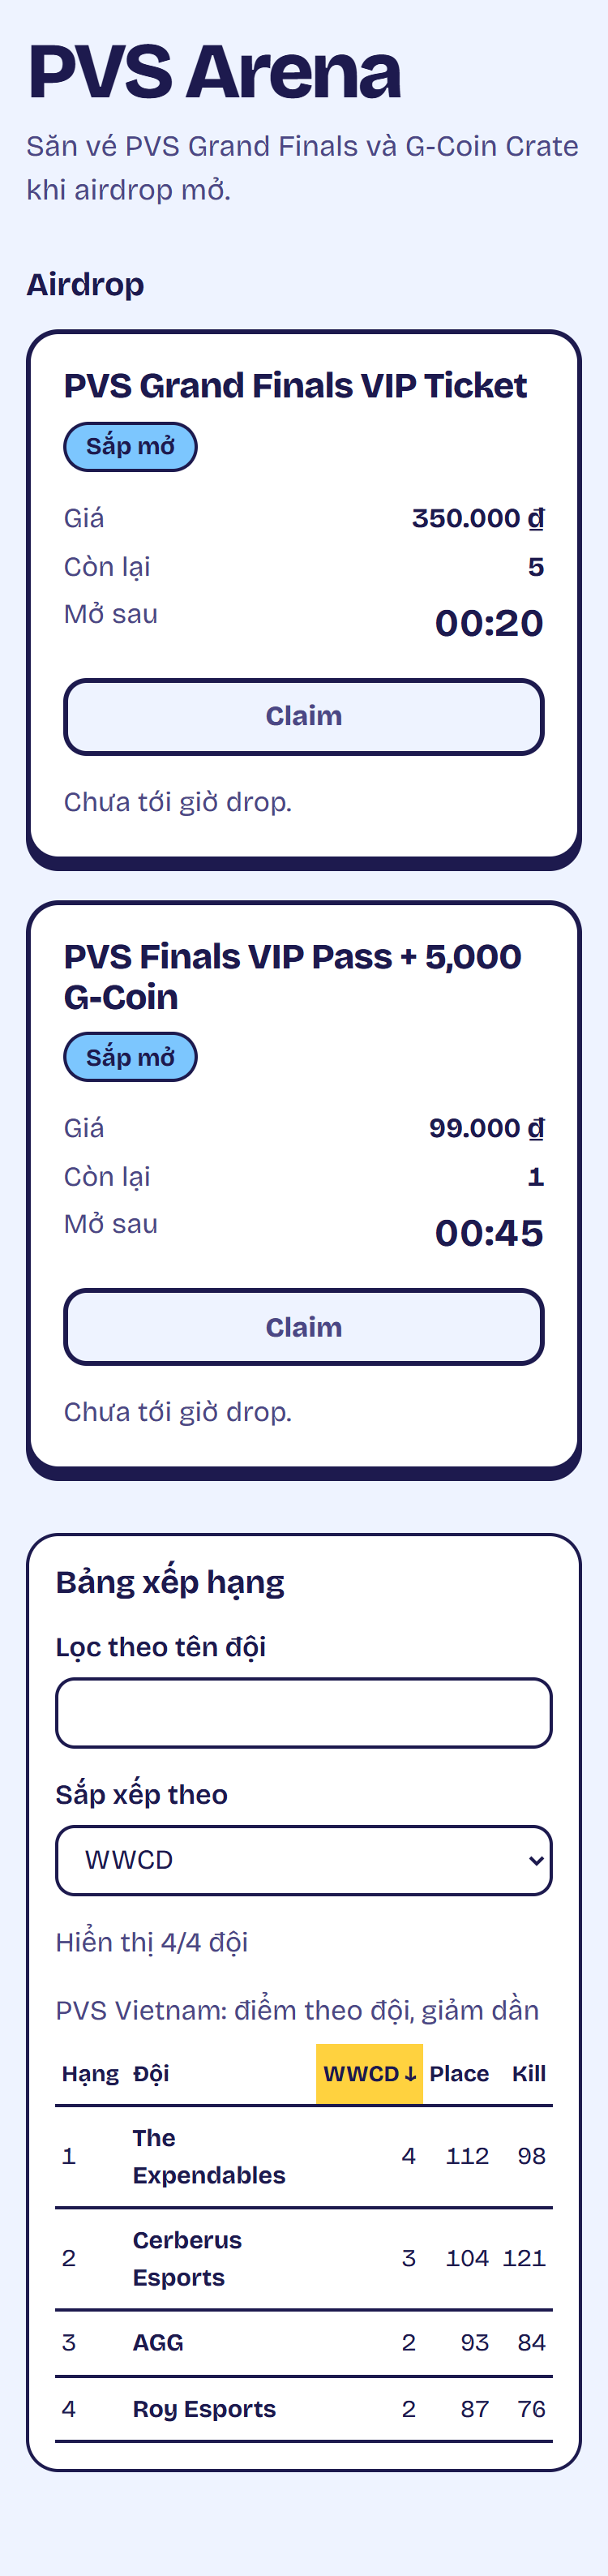
\includegraphics[width=0.3\textwidth,trim=0 1000bp 0 0,clip]{images/hw3_375.png}
    \caption{375 px (top of the page): countdown, VND price, disabled Claim with a reason}
    \label{fig:hw3-375}
\end{figure}

\evfig{hw3_409.png}{0.3}{Claim rejected with 409: stock returns to its old value and an alert explains why}{fig:hw3-409}
\evfig{hw3_lighthouse.png}{0.9}{Lighthouse: Performance 100, Accessibility 100, Best Practices 100}{fig:hw3-lh}
\evfig{hw3_a11y.png}{0.9}{Accessibility tree of the Claim button}{fig:hw3-a11y}

\section{Verification}

\begin{table}[H]
\centering
\begin{tabular}{L{5.5cm} L{7.5cm}}
\toprule
\textbf{Check} & \textbf{Result} \\
\midrule
\texttt{npm test} & 7 files, 61 tests pass \\
\texttt{npm run lint} & Clean \\
Hidden tab 330 s & Displayed 04:29, drift 0 s (before and after wake) \\
409 rollback & Stock 1 $\rightarrow$ 0 $\rightarrow$ 1, alert shown \\
Horizontal scroll, 320 and 375 px & None \\
Contrast & 14/14 pairs pass, lowest 6.24:1 \\
Claim transition & 0.07 s; 0 s with reduced motion \\
Lighthouse & 100 / 100 / 100 \\
\bottomrule
\end{tabular}
\caption{Homework 3 results}
\label{tab:hw3-verify}
\end{table}

Not done: screen reader test; Lighthouse SEO was not run.

\section{AI Failure Audit}

\begin{itemize}
    \item Test runner reported as flaky''; the real cause was running \texttt{npm test} from the wrong folder (error 6).
    \item Countdown \texttt{<output>} was a live region announcing every second (error 7).
\end{itemize}

\section{Source Code}

\begin{center}
    \href{https://github.com/Prosperum26/24520626_QuangPhuHung_MSIS207_Lab03/tree/main/src/homeworks/KraftonPubgVnArena}
    {\textbf{View Homework 3 on GitHub}}

    \href{https://github.com/Prosperum26/24520626_QuangPhuHung_MSIS207_Lab03/blob/main/AI_FAILURE_AUDIT.md}
    {\textbf{View AI failure audit on GitHub}}
\end{center}

\chapter{Submission \& Resources}
\label{chap:submission-resources}

\begin{center}
    \href{https://github.com/Prosperum26/24520626_QuangPhuHung_MSIS207_Lab03}
    {\texttt{24520626\_QuangPhuHung\_MSIS207\_Lab03}}
\end{center}

\begin{itemize}
    \item \textbf{Tests:} 347 pass in total (HW1 146, HW2 140, HW3 61); lint clean in all three.
    \item \textbf{Prompt logs:} \texttt{docs/prompt\_logs/}
    \item \textbf{AI failure audit:} \texttt{AI\_FAILURE\_AUDIT.md}
    \item \textbf{Evidence:} \texttt{evidence/} in each homework folder
    \item \textbf{Limits:} no screen reader testing; HW1 and HW2 still lack some 375 px and keyboard screenshots.
\end{itemize}

\begin{center}
\textbf{END}
\end{center}

\end{document}
